\subsection{Figuras de apoyo}
\label{anx:figuras}

En este anexo se reúnen las figuras a las que remiten los capítulos V y VII.

\begin{figure}[!htb]
\centering
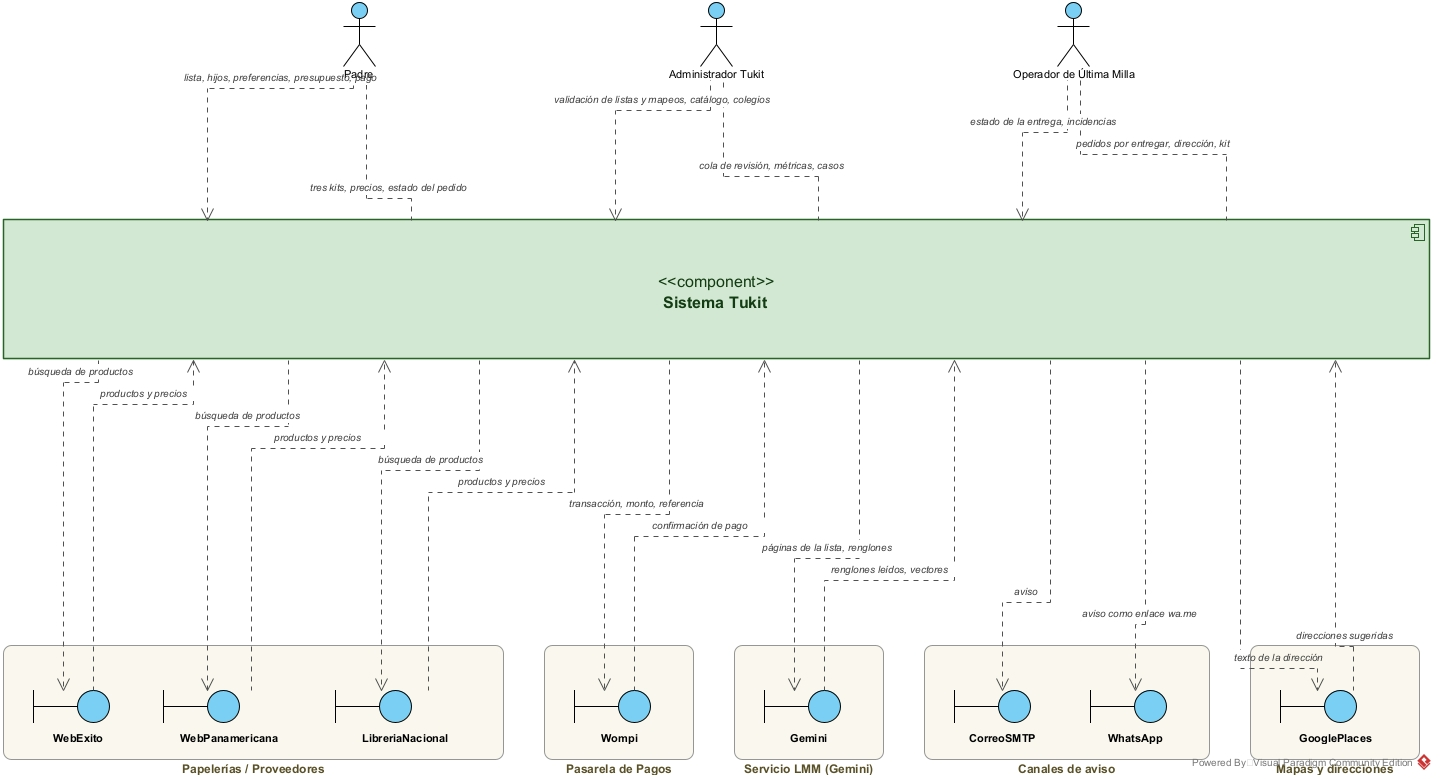
\includegraphics[width=\textwidth]{img/modelo/contexto.jpg}
\caption[Vista de contexto: Tukit frente a sus actores y sistemas externos.]{Vista de contexto,
en notación UML: Tukit frente a sus actores (el padre es el acudiente) y a los sistemas externos,
agrupados por función. Cada flecha lleva la información que pasa entre las partes.}
\label{fig:c4-contexto}
\end{figure}

\input{\graficasdir/F3-2.tex}

\input{\graficasdir/F5-2.tex}

\begin{figure}[!htb]
\centering
\resizebox{\textwidth}{!}{% Vista de despliegue: cómo corre Tukit en el portátil del equipo (make arriba / reanudar / backend),
% con el túnel de Cloudflare de las sesiones con acudientes. Misma paleta que c4-contenedores.tex.
\definecolor{tkPerF}{HTML}{FFF0B8}\definecolor{tkPerB}{HTML}{9A7B00}
\definecolor{tkAppF}{HTML}{CFE2F7}\definecolor{tkAppB}{HTML}{1F4E86}
\definecolor{tkProcF}{HTML}{D3EDD0}\definecolor{tkProcB}{HTML}{2E6B2B}
\definecolor{tkExtF}{HTML}{FAD7B5}\definecolor{tkExtB}{HTML}{A8500F}
\definecolor{tkInfF}{HTML}{DEDEDE}\definecolor{tkInfB}{HTML}{4D4D4D}
\definecolor{tkBdF}{HTML}{CDEBEB}\definecolor{tkBdB}{HTML}{1C6E6E}
\definecolor{tkMqF}{HTML}{E2D6F4}\definecolor{tkMqB}{HTML}{5B2E99}
\begin{tikzpicture}[x=1cm, y=1cm, font=\scriptsize,
  per/.style={draw=tkPerB, thick, rounded corners=7pt, align=center, fill=tkPerF, inner sep=3pt, minimum height=7mm},
  cont/.style={draw=tkAppB, rounded corners=2pt, align=center, fill=tkAppF, inner sep=2pt, minimum height=8mm},
  proc/.style={draw=tkProcB, rounded corners=2pt, align=center, fill=tkProcF, inner sep=2pt, minimum height=7mm},
  ext/.style={draw=tkExtB, rounded corners=2pt, align=center, fill=tkExtF, inner sep=2pt, minimum height=7mm},
  infra/.style={draw=tkInfB, rounded corners=2pt, align=center, fill=tkInfF, inner sep=2pt, minimum height=7mm},
  bd/.style={draw=tkBdB, cylinder, shape border rotate=90, aspect=0.22, align=center, fill=tkBdF, inner sep=2pt},
  mq/.style={draw=tkMqB, rounded corners=2pt, align=center, fill=tkMqF, inner sep=2pt, minimum height=7mm},
  nodo/.style={draw=black!55, rounded corners=3pt, fill=black!4},
  http/.style={-{Stealth[length=1.6mm]}, semithick},
  rot/.style={font=\tiny, fill=white, inner sep=1pt}]
% Visitante
\node[per, text width=3.2cm] (acudiente) at (1.8,0) {\textbf{Acudiente}\\navegador del celular};
\node[ext, text width=3.2cm] (tunel) at (1.8,-1.7) {\textbf{Túnel de Cloudflare}\\URL temporal, solo en las sesiones};
% Portátil
\draw[nodo] (3.9,0.6) rectangle (15.1,-9.1);
\node[anchor=north west, font=\scriptsize\bfseries] at (4.0,0.5) {Portátil del equipo (127.0.0.1)};
\node[cont, text width=3.0cm] (web) at (5.6,-1.0) {\textbf{Aplicación web}\\Next.js, puerto 3000};
\node[cont, text width=3.0cm] (admin) at (9.0,-1.0) {\textbf{Panel de administración}\\Next.js, puerto 3001};
\node[cont, text width=10.4cm] (gateway) at (9.4,-2.5) {\textbf{Puerta de enlace}, puerto 8010};
\node[cont, text width=1.6cm] (s1) at (5.0,-4.0) {\textbf{Identidad}\\8011};
\node[cont, text width=1.6cm] (s2) at (7.0,-4.0) {\textbf{Catálogo}\\8012};
\node[cont, text width=1.6cm] (s3) at (9.0,-4.0) {\textbf{Inteligencia}\\8013};
\node[cont, text width=1.6cm] (s4) at (11.0,-4.0) {\textbf{Comercio}\\8014};
\node[cont, text width=1.6cm] (s5) at (13.0,-4.0) {\textbf{Operación}\\8015};
\node[proc, text width=10.4cm] (fondo) at (9.4,-5.3) {Procesos en segundo plano de cada servicio (trabajador, publicadores, sondeadores, barredor, repartidor)};
\node[infra, text width=3.4cm] (pg) at (5.9,-7.0) {\textbf{PostgreSQL 16 con pgvector}\\5 bases, puerto 5432};
\node[mq, text width=2.8cm] (mq) at (9.4,-7.0) {\textbf{RabbitMQ}\\AMQP 5672, consola 15672};
\node[infra, text width=2.3cm, densely dotted] (redis) at (12.1,-7.0) {\textbf{Redis}\\opcional};
\node[infra, text width=1.9cm, densely dotted] (jaeger) at (14.1,-7.0) {\textbf{Jaeger}\\opcional};
\node[anchor=north west, text width=10.9cm, align=left, font=\scriptsize, inner sep=0pt] at (4.2,-7.9)
  {Un comando levanta los procesos, otro los vuelve a levantar tras un apagado y un tercero migra, siembra y levanta de cero.};
% Servicios externos
\node[ext, text width=3.2cm] (wompi) at (1.8,-4.4) {\textbf{Wompi}\\modo simulado; no sale a la red};
\node[ext, text width=3.2cm] (gemini) at (1.8,-6.5) {\textbf{Gemini}\\lectura de listas y vectores};
\node[ext, text width=3.2cm] (otros) at (1.8,-8.3) {\textbf{OpenStreetMap, correo y tiendas}\\llamadas salientes};
% Flechas
\draw[http] (acudiente) -- (tunel);
\draw[http] (tunel.east) -- ++(0.3,0) |- (web.west);
\draw[http] (web.east) -- (admin.west);
\draw[http] (web.south) -- ++(0,-0.35) -| ([xshift=-3.5cm]gateway.north);
\draw[http] (admin.south) -- (admin.south |- gateway.north);
\foreach \s in {s1,s2,s3,s4,s5}{\draw[http] (\s.north |- gateway.south) -- (\s.north);}
\draw[http] (s3.south) -- (s3.south |- fondo.north);
\draw[http] (fondo.south) -- (fondo.south |- mq.north);
\draw[http] (fondo.south -| pg.north) -- (pg.north);
\draw[http, dashed] (s3.west) -- ++(-2.7,0) |- (gemini.east);
\draw[http, dashed, densely dotted] (wompi.east) -- ++(0.2,0) |- (s4.west);
\end{tikzpicture}
}
\caption[Vista de despliegue: cómo corre Tukit en el equipo.]{Vista de despliegue. Todo el
sistema corre en un portátil: dos aplicaciones web, la puerta de enlace, cinco servicios,
sus procesos en segundo plano y la infraestructura (PostgreSQL, RabbitMQ, y Redis y Jaeger
opcionales). En las sesiones con acudientes se abre un túnel de Cloudflare hacia la aplicación
web, y Wompi funciona en modo simulado. Misma paleta que la Figura~\ref{fig:c4-contenedores}.}
\label{fig:despliegue}
\end{figure}

\begin{figure}[!htb]
\centering
\begin{tabular}{cc}
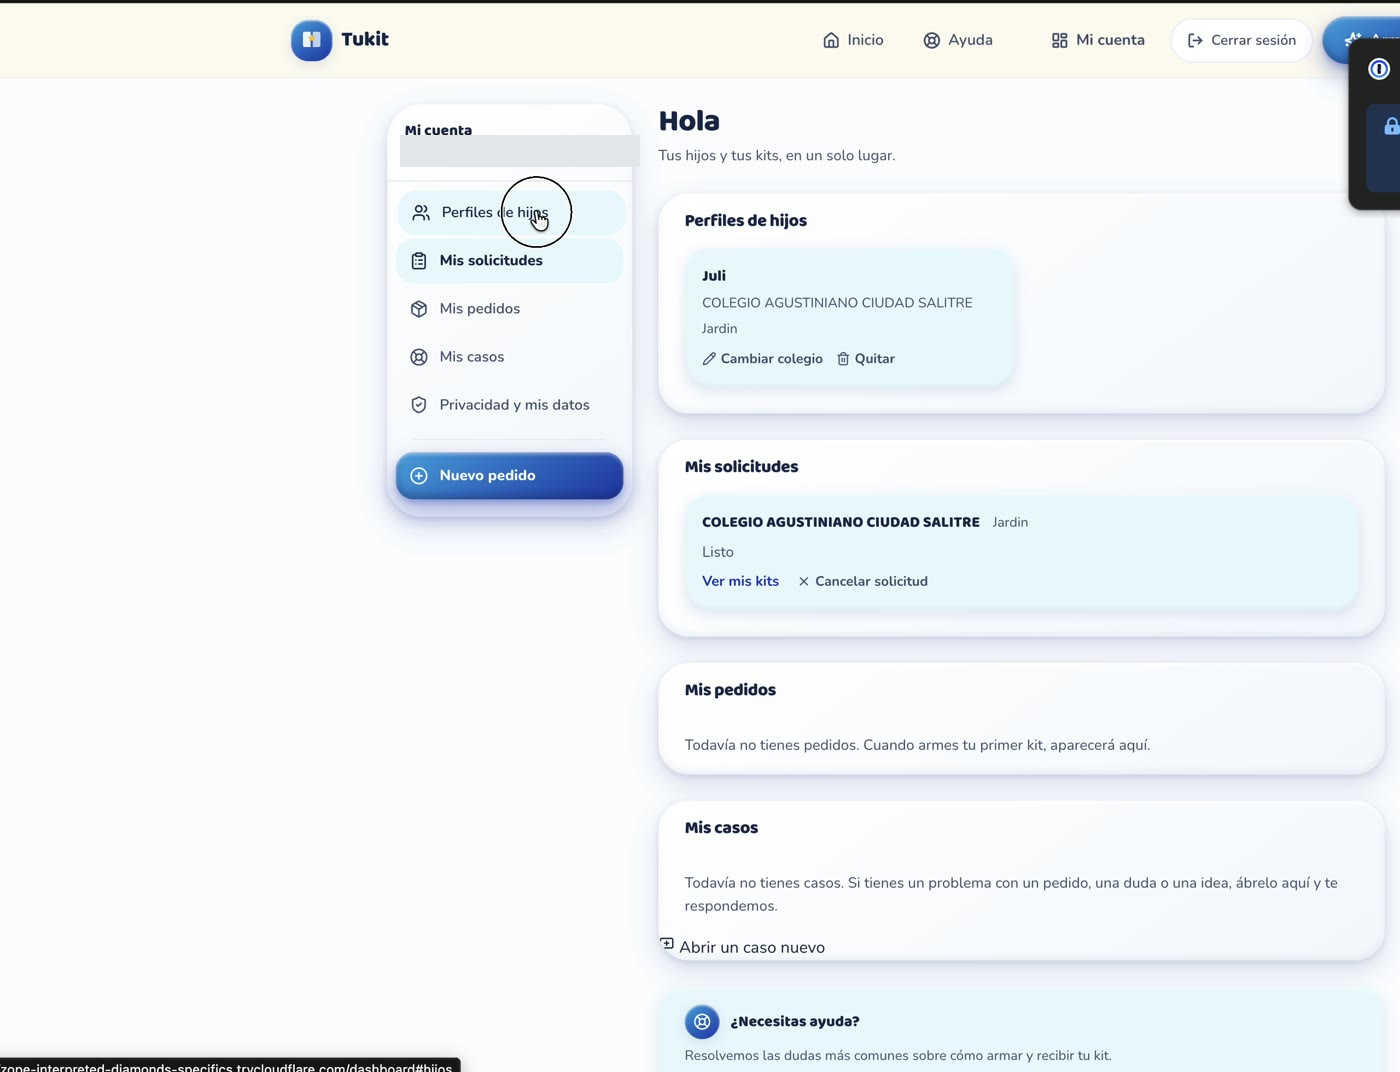
\includegraphics[width=0.47\textwidth]{img/producto/cuenta.jpg} &
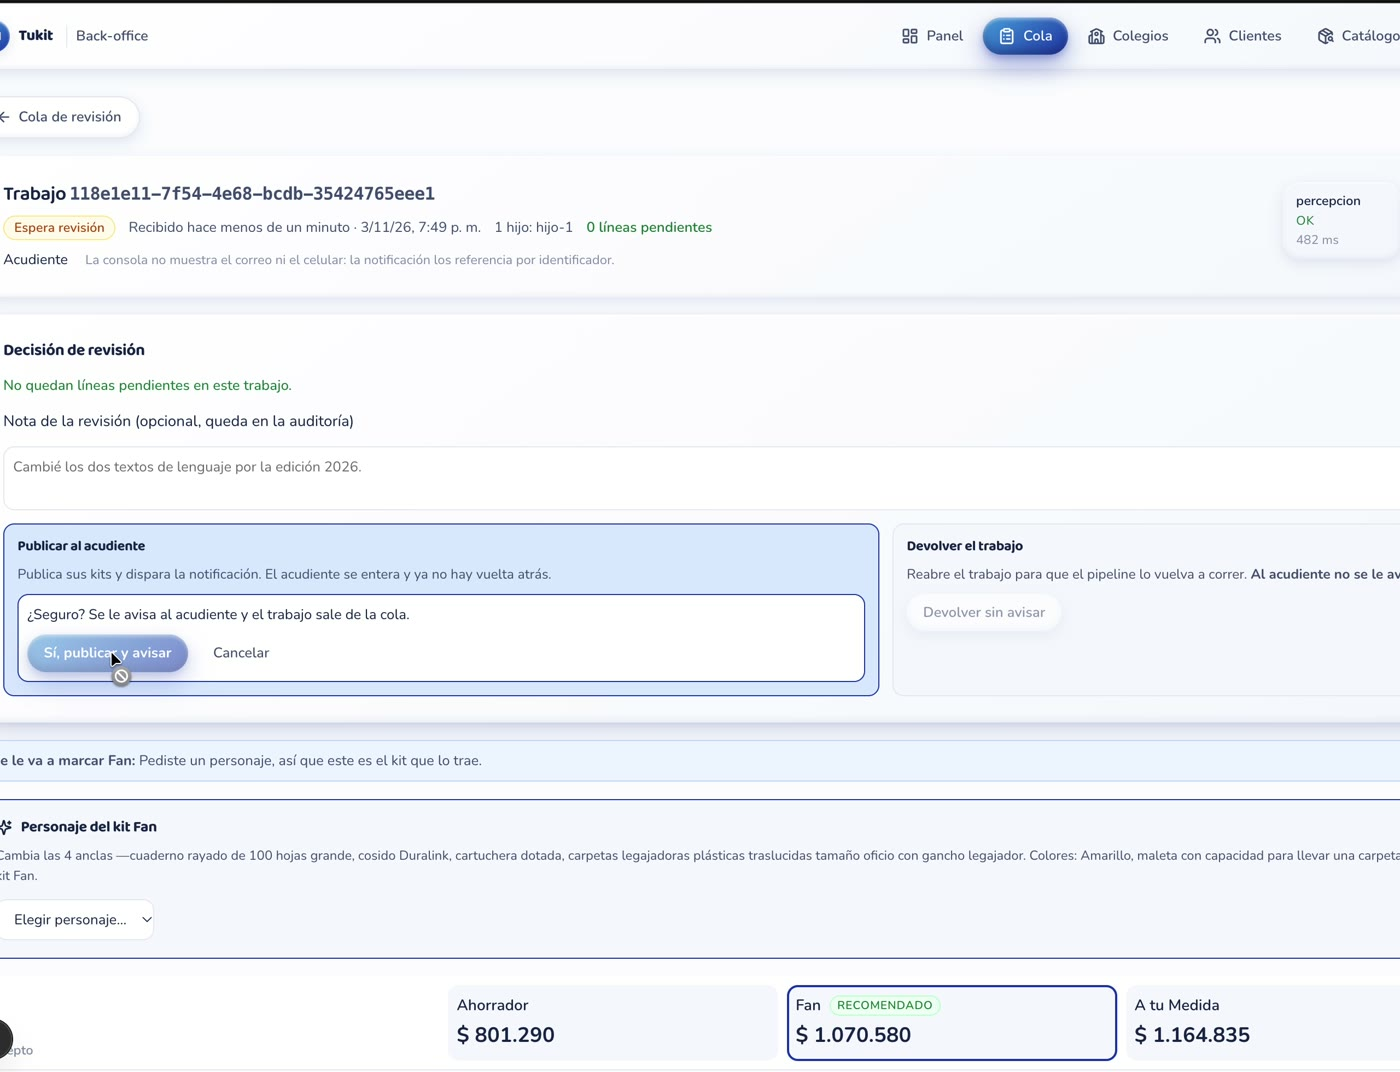
\includegraphics[width=0.47\textwidth]{img/producto/revision.jpg} \\
\footnotesize (a) La cuenta del acudiente & \footnotesize (b) Revisión del kit en el panel del equipo \\
\end{tabular}
\caption[Cuenta del acudiente y revisión del equipo.]{La cuenta del acudiente, con sus hijos,
solicitudes, pedidos y casos (a), y la revisión de un kit en el panel de administración antes de
publicarlo al acudiente (b). Capturas de la versión usada en el OE5.}
\label{fig:producto-equipo}
\end{figure}
